\chapter{Graphics Match, το Πρώτο μας Γραφικό Παιχνίδι}
\label{chap:graphics-match}
%
\section{Εισαγωγή}
%
Υπομείνατε παιχνίδια με αριθμούς και text adventures, αντέξατε να μάθετε τόσα στοιχεία και εντολές της python. Μόνο στο προηγούμενο κεφάλαιο φάνηκε μια μικρή αχτίδα φωτός: σας δείξαμε επιτέλους γραφικό προγραμματισμό και pygame! Χρειάστηκε βέβαια να μάθετε πολλά νέα πράγματα -- και ελπίζουμε να έχετε κατανοήσει τα περισσότερα. Ας συνοψίσουμε λίγο κάποια βασικά:
%
\begin{itemize}
\item[-] Τα παιχνίδια σε pygame είναι {\em event driven}, οδηγούνται δηλ. από συμβάντα. Συμβάν είναι όταν πιέσετε το close. Συμβάν είναι όταν το πρόγραμμα σας πρέπει να ανταποκριθεί σε κάποιο πλήκτρο που πίεσε ο χρήστης.
\item[-] Το παιχνίδι αποτελείται πάντα από ένα βασικό βρόχο που εκτελείται συνέχεια μέχρι να το τερματίσουμε. Μέσα σε αυτό το βρόχο δημιουργούμε αρχικά το κάθε καρέ μας σε μια προσωρινή μνήμη και στη συνέχεια (με μια μόνο εντολή) το μεταφέρουμε στην ορατή οθόνη.
\item[-] Για να γίνει η μεταφορά χρειαζόμαστε την εντολή {\tt pygame.display.update()}
Βασικές έννοιες στην δημιουργία του κειμένου ή των γραφικών μέσα στο παράθυρο μας είναι η {\em επιφάνεια (surface)} και η μέθοδος {\tt blit}.
\item[-] Κάθε φορά που εκτελείται ο κύριος βρόχος εμφανίζεται ένα καρέ. Όσο πιο γρήγορα γίνεται η εκτέλεση τόσα περισσότερα καρέ το δευτερόλεπτο θα δείχνουμε -- εκτός αν τα περιορίσουμε εμείς.
\end{itemize}
%
Στο Κεφάλαιο \ref{chap:objects-intro} συνειδητοποιήσαμε ότι η python είναι αντικειμενοστραφής γλώσσα και βολεύει για παιχνίδια.

Η υπομονή σας επιτέλους θα ανταμειφθεί: θα φτιάξουμε το πρώτο μας κανονικό γραφικό παιχνίδι! Ένα πρόγραμμα που θα συνδυάζει πολλά από αυτά που μάθαμε μέχρι τώρα. Η υλοποίηση βέβαια είναι το τελευταίο μόνο κομμάτι του puzzle -- το βασικό είναι να σκεφτούμε τον αλγόριθμο και τα δεδομένα μας.
%
\section{Graphics Match -- Η Σύγχρονη Εκδοχή}
%
Το πρόγραμμα που θα φτιάξουμε ονομάζεται Graphics Match και είναι η σύγχρονη εκδοχή του προγράμματος για TI-99/4A που υπάρχει από το 1981! Από τη φωτογραφία καταλαβαίνετε ότι πρόκειται για ένα απλό παιχνίδι slot machine με φρουτάκια (και μπάρες, καμπάνες κλπ). Μόλις μάλιστα το τρέξετε θα αρχίσετε να αμφιβάλλετε για την έννοια των ``τυχερών'' παιχνιδιών. Μάλλον ``άτυχα'' θα έπρεπε να τα λένε. Ναι, ακόμα και στην python εκδοχή τους, χάνει κανείς συνέχεια!

\begin{SCfigure}
  \centering
  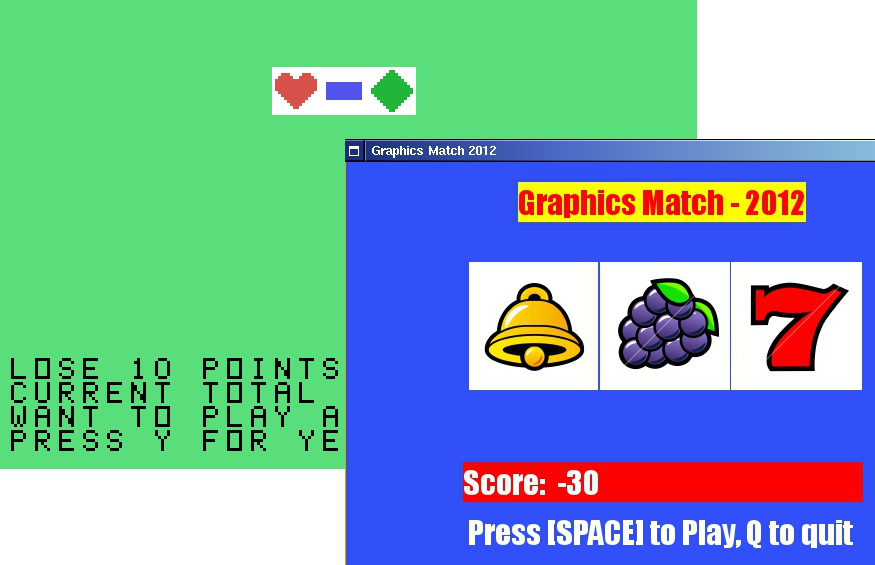
\includegraphics[width=0.6\textwidth]{images/chapter6/graphics-match}
  \caption[Graphics Match, Παλιό και Νέο]{Το παλιό και το καινούριο Graphics Match. Φαίνεται ξεκάθαρα ότι
τα γραφικά του 1984 αποτελούνται από χαρακτήρες που έχουμε επανακαθορίσει.
Το άλλο που φαίνεται ξεκάθαρα είναι ότι\ldots{} χάνουμε! Καλύτερα να
επενδύσετε σε γραμμάτια του Ελληνικού Δημοσίου παρά να προσπαθείτε να
κερδίσετε το Graphics Match!}
  \label{6-1}
\end{SCfigure}
%
\subsection{Ιστορία και Θεωρία}
%
Το ``ταίριασμα των γραφικών'' πρωτοεμφανίστηκε στο βιβλίο User's Reference Guide του ΤΙ-99/4Α και ίσως να είναι το πρώτο παιχνίδι που (αντ)έγραψα ποτέ! Σαν λογική δεν είναι ιδιαίτερα δύσκολο και σύντομα έφτιαξα αρκετά πιο πολύπλοκα παιχνίδια μόνος μου. Μου έδωσε όμως μερικές καλές ιδέες και με δίδαξε κάποια πράγματα που πρέπει να αποφεύγω.

Την εποχή του πρωτότυπου Graphics Match δεν υπήρχε Internet για να κατεβάσει κανείς εικόνες και γραφικά. Έπρεπε όλα να τα δημιουργούμε μόνοι μας, στο χέρι ή με κάποιο δικό μας πρόγραμμα. Για να καταλάβετε, τα γραφικά ορίζονταν σαν χαρακτήρες. Καθένα από τα φρουτάκια αποτελούνταν από τέσσερις χαρακτήρες σε μια μήτρα 2Χ2. Είχαμε τη δυνατότητα να αλλάζουμε τη μορφή των χαρακτήρων, κάτι σαν σημερινή σχεδίαση γραμματοσειρών αλλά σε πολύ απλή μορφή.

Το παιχνίδι μας χρησιμοποιεί έξι σύμβολα συνολικά.

\begin{table}[H]
\begin{center}
\begin{tabular}{|c|l|}
\hline
\textbf{Αριθμός} & \textbf{Σύμβολο} \\
\hline
0 & Λεμόνι \\
\hline
1 & Μπάρα \\
\hline
2 & Κεράσι \\
\hline
3 & Καμπανάκι \\
\hline
4 & Βατόμουρο \\
\hline
5 & Το 7 (μη με ρωτήσετε γιατί) \\
\hline
\end{tabular}
\end{center}
\caption{Τα γραφικά του παιχνιδιού}
\label{t6-1}
\end{table}

\begin{figure}
  \centering
  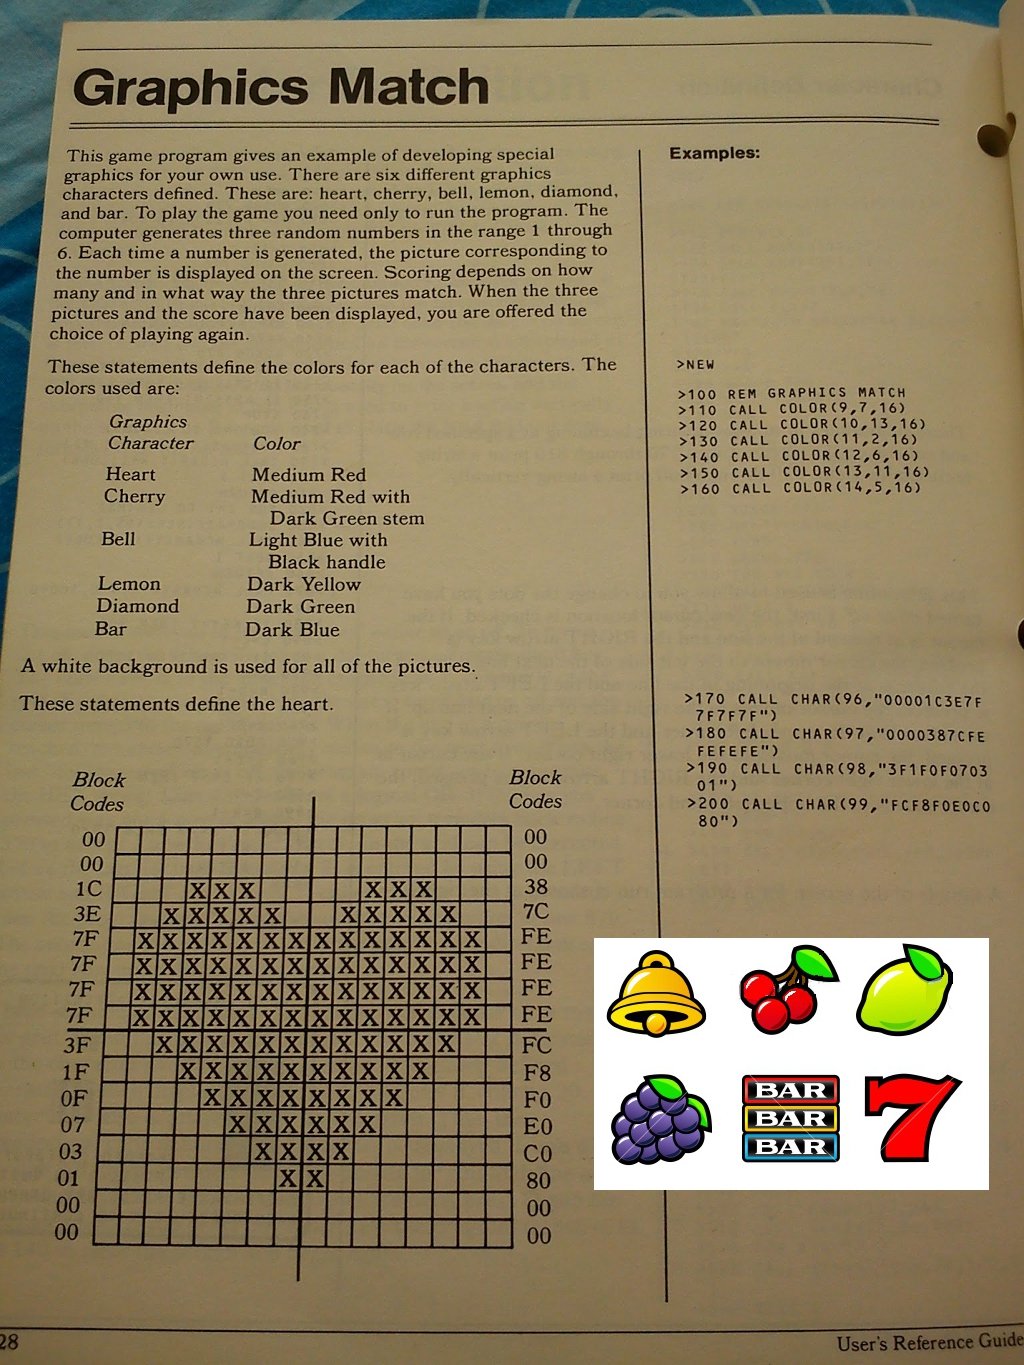
\includegraphics[height=0.95\textheight, angle=90]{images/chapter6/usersguide}
  \caption[TI-BASIC και Graphics Match]{Το αρχικό πρόγραμμα Graphics Match, εμφανίζεται σε TI BASIC στο
User's Reference Guide του ΤΙ-99/4Α το 1981. Ένα από τα πρώτα παιχνίδια που
θα δοκίμαζε κανείς να γράψει μόλις αγόραζε αυτό τον υπολογιστή. Στο listing
φαίνεται καθαρά πως ορίζονται οι τέσσερις χαρακτήρες που αποτελούν κάθε
σύμβολο. Και ναι, όπως βλέπετε το gimp των 80s απαιτεί τη γνώση δεκαεξαδικού
συστήματος! Συγκρίνετε το με τις έτοιμες εικόνες που χρησιμοποιούμε στο δικό
μας πρόγραμμα. {\bf Σημείωση:} Γυρίστε το βιβλίο στο πλάι :)}
  \label{6-2}
\end{figure}

Το gameplay έχει ως εξής: Με την εκκίνηση του παιχνιδιού, τρία σύμβολα  εναλλάσσονται γρήγορα σε μια γραμμή. Οι εναλλαγές σταματάνε μετά από 50 φορές και ανάλογα με τα σύμβολα που φαίνονται στη γραμμή υπολογίζεται ένα score. Ο τρόπος υπολογισμού είναι ο παρακάτω:

\begin{itemize}
\item[-] Τρία όμοια σύμβολα σε μια γραμμή -- Jackpot! Κερδίζετε 75 βαθμούς.
\item[-] Τα δύο πρώτα σύμβολα όμοια: Αν είναι λεμόνια, μπάρες ή κεράσια κερδίζετε 40 βαθμούς, αν είναι οτιδήποτε άλλο 10 βαθμούς.
\item[-]Το πρώτο και το τρίτο σύμβολο όμοια: κερδίζετε 10 βαθμούς.
\item[-]Το πρώτο και το δεύτερο όμοια ή τίποτα όμοιο, χάνετε 10 βαθμούς.
\end{itemize}
%
Φαντάζομαι μαντέψατε ποια περίπτωση είναι αυτή που τυχαίνει περισσότερο ε\ldots{} :)

Τώρα, σε αντίθεση με το αρχικό πρόγραμμα του 1981, δεν χρειάζεται πλέον (ευτυχώς!) να σχεδιάσουμε εμείς τα λεμόνια, τα κεράσια τα καμπανάκια και όλα αυτά τα αστεία σύμβολα γενικά. Γιατί αρκεί να βρούμε αντίστοιχες εικόνες σε κατάλληλο μέγεθος από το Internet. Και δεν ξέρω αν το έχετε παρατηρήσει, αλλά υπάρχουν αρκετά ``Internet καζίνο'' από τα οποία μπορούμε να πάρουμε τα γραφικά! Πιστέψτε με, το μόνο πράγμα που θα πάρετε ποτέ από αυτά τα sites είναι αυτά τα γραφικά. Αν περιμένετε λεφτά, σωθήκατε.

Το καλό με τις έτοιμες εικόνες είναι ότι έχουν όλες το ίδιο στυλ και μέγεθος
αφού προορίζονται για το συγκεκριμένο παιχνίδι -- και αυτό μας βολεύει αφάνταστα. No photoshopping (ή\ldots{} gimping) required!

Μόλις εμφανιστεί το score, ο χρήστης πιέζει το {\tt SPACE} αν θέλει να ξαναπαίξει ή το {\tt Q} για να τερματίσει το παιχνίδι. Το παιχνίδι φυσικά τερματίζεται και αν ο χρήστης κλείσει το παράθυρο από το close. Ξέχασα να σας πω ότι αρχικά ξεκινάτε με μηδέν βαθμούς και είναι πολύ πιθανό όταν το βαρεθείτε να φύγετε με\ldots{} -1000. Αν παίξετε πολύ ώρα μπορεί να χρειαστείτε και τη βοήθεια του ΔΝΤ για να\ldots{} ξελασπώσετε :)
%
\subsection{Ο Αλγόριθμος}
%
Ξεχάστε και την python και το pygame για την ώρα. Ας επικεντρωθούμε στο πως λειτουργεί αυτό το παιχνίδι και τι θα περιέχει ο βασικός βρόχος σε γενική μορφή.

Μια και έχουμε ήδη κάνει μια δυναμική εκκίνηση στον αντικειμενοστραφή προγραμματισμό ας το σκεφτούμε λίγο με αυτή τη λογική. Το πως θα την υλοποιήσουμε είναι μια άλλη ιστορία!

Φανταστείτε λοιπόν ότι έχετε δημιουργήσει μια κλάση για τη γραμμή με τα τρία περιστρεφόμενα φρουτάκια. Τι θα έπρεπε να περιέχει; Τουλάχιστον τρία πράγματα:
%
\begin{itemize}
\item Μια συνάρτηση constructor που να κατασκευάζει ένα αντικείμενο αυτού του είδους. Ο constructor είναι μια καλή ευκαιρία να φορτώσουμε και τις εικόνες.
\item Μια μέθοδο {\tt Spin} που να κάνει τα φρουτάκια να εναλλάσσονται πάνω σε μια επιφάνεια σε συγκεκριμένες συντεταγμένες που θα δώσουμε και ενδεχομένως με συγκεκριμένο framerate.
\item Μια μέθοδο {\tt GetScore} που θα την καλούμε για να μας επιστρέφει πόσο\ldots{} χάσαμε.
\end{itemize}
%
Προσέξτε το μαγικό τρικ τώρα: υποθέστε ότι όλα αυτά τα έχουμε φτιάξει και λειτουργούν! Ποιο θα ήταν το πρόγραμμα μας στον κύριο βρόχο σε γενικές γραμμές;

Ας υποθέσουμε ότι έχουμε ονομάσει την κλάση {\tt Spinner} και θέλουμε να δημιουργήσουμε ένα αντικείμενο αυτής της κλάσης. Αυτό θα γίνονταν κάπως έτσι:

\begin{minted}[bgcolor=bg, frame=lines, framesep=10pt]{python}
slotmachine = Spinner()
\end{minted}

\begin{figure}
\centering
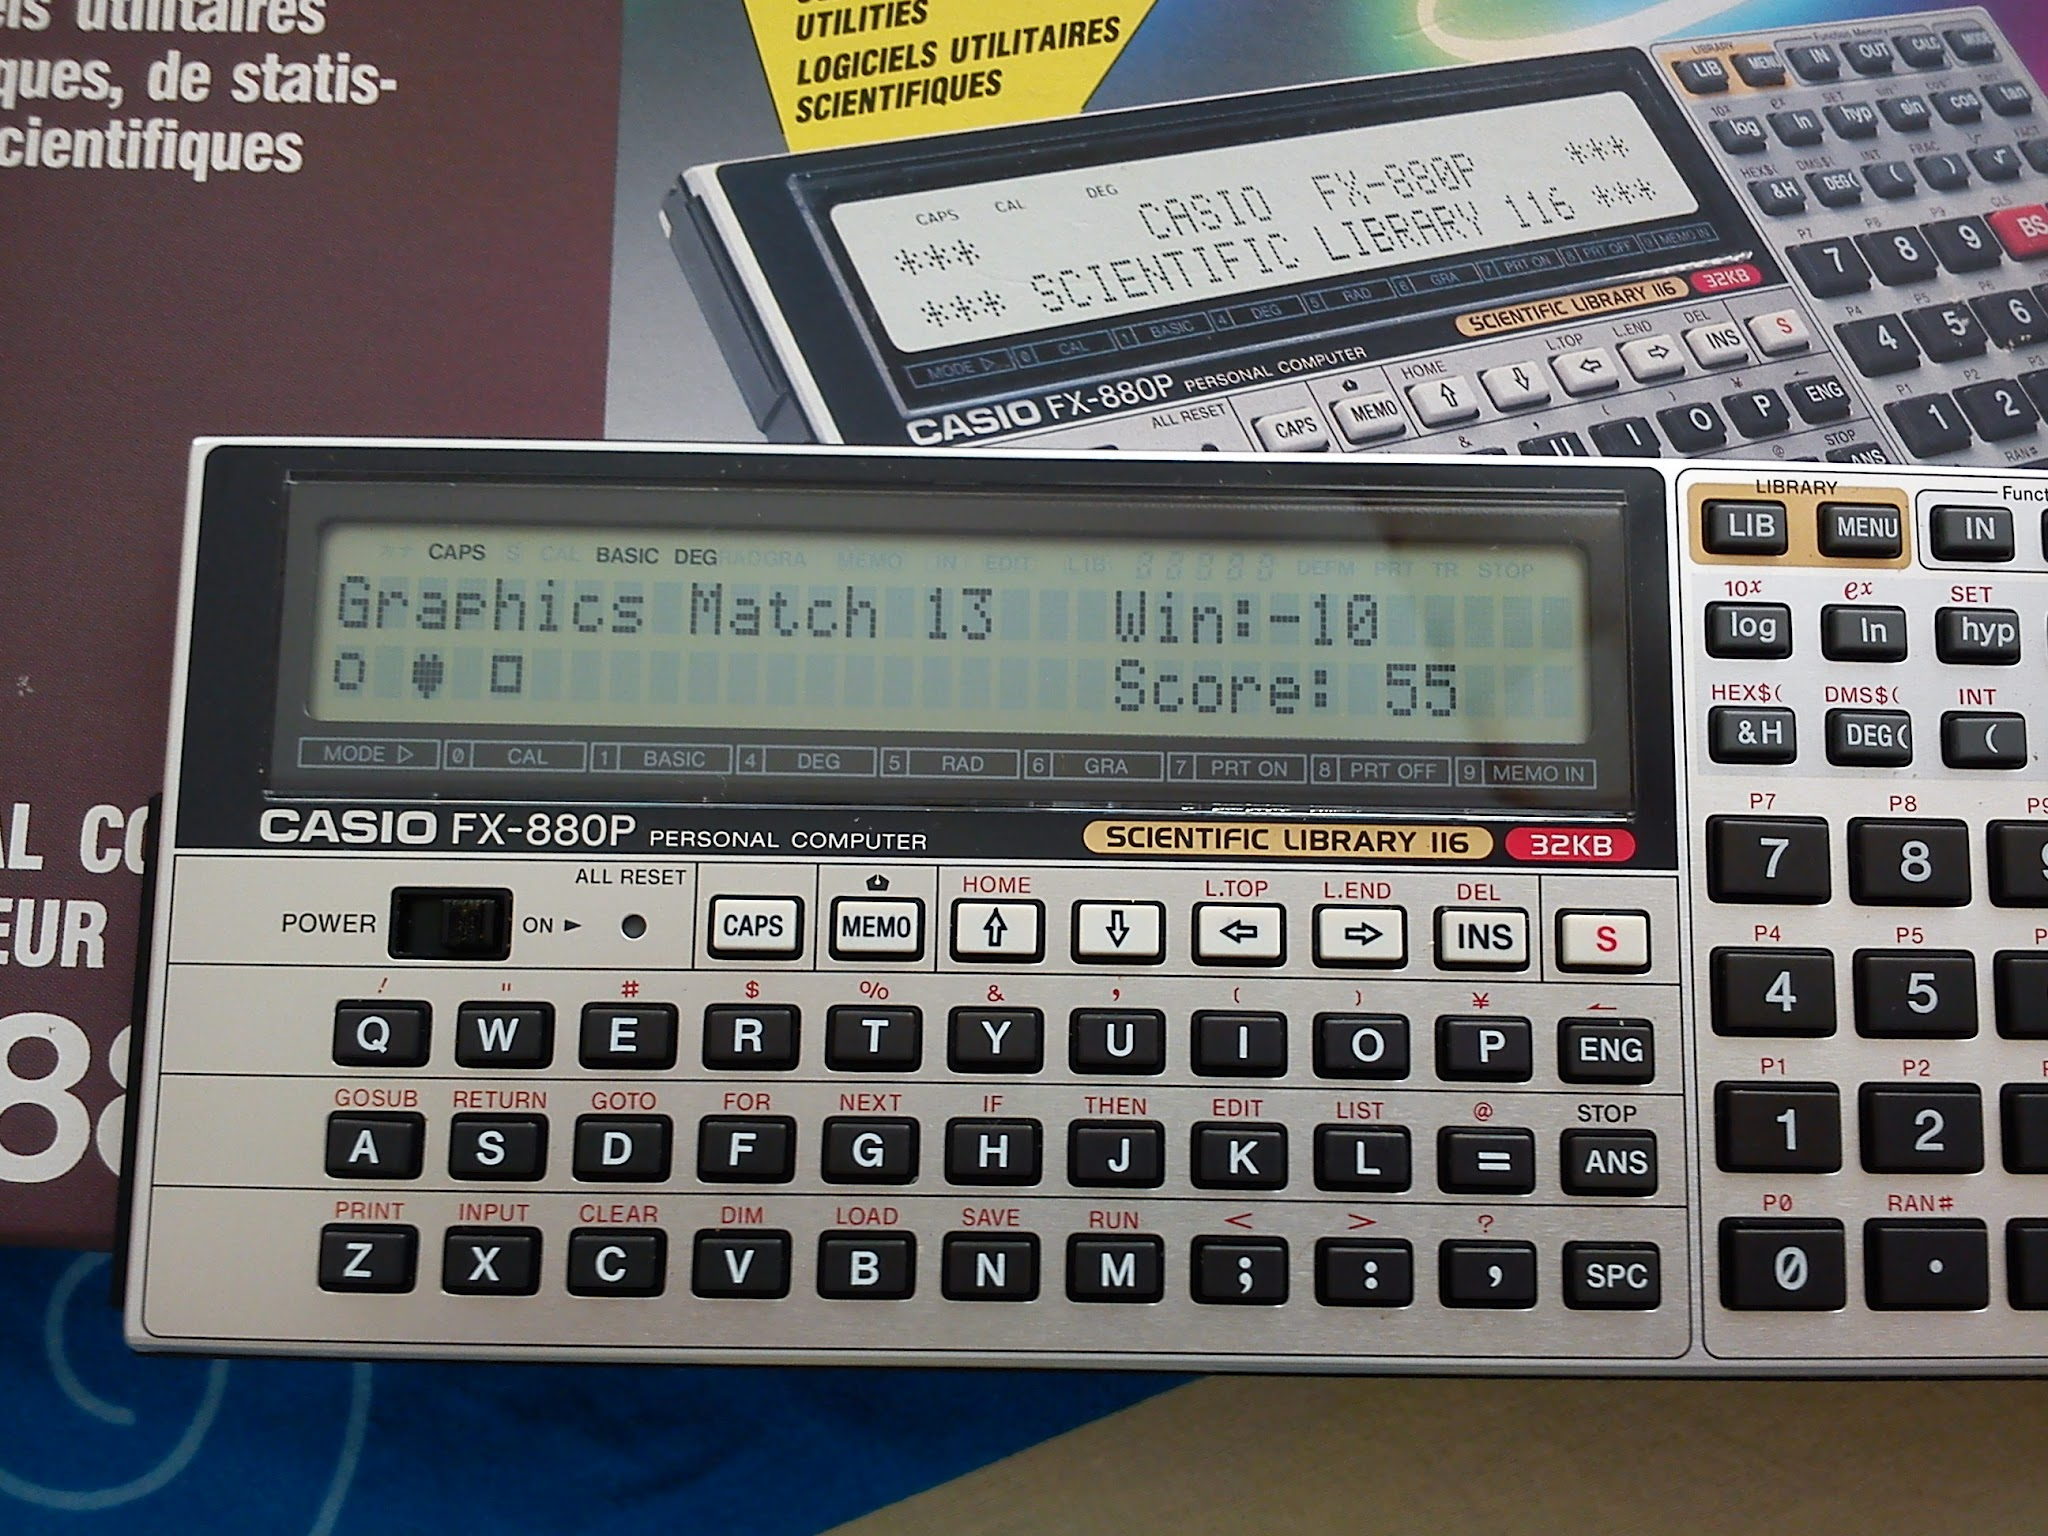
\includegraphics[height=0.8\textheight]{images/chapter6/fx880}
\caption[CASIO FX-880P και Graphics Match]{Ποιος σας είπε ότι το παιχνίδι περιορίζεται μόνο στον ΤΙ και στην
python που έχετε μπροστά σας; O pocket υπολογιστής που βλέπετε μπροστά σας,
το διάσημο Casio FX-880P (από τους καλύτερους BASIC programmable που έβγαλε
ποτέ η CASIO) έχει εξαιρετική γλώσσα προγραμματισμού κατάλληλη για να
γράψουμε ακόμα και παιχνίδια.  Και μην ανησυχείτε καθόλου: χάνει κανείς με
την ίδια συχνότητα και σε αυτό το σύστημα!}
\label{6-3}
\end{figure}

Έτσι θα κληθεί ο constructor του {\tt Spinner} και θα δημιουργηθεί το
αντικείμενο {\tt slotmachine}. Βέβαια στο συγκεκριμένο constructor θέλουμε να δώσουμε και κάτι ακόμα (τις εικόνες) αλλά αυτό είναι μια τεχνική λεπτομέρεια που θα φροντίσουμε αργότερα. Ο κύριος βρόχος, σε μορφή --- περίπου --- ψευδοκώδικα θα είναι κάτι σαν το παρακάτω:
%
\begin{verbatim}
score = 0
endgame = False
spacepressed = True
while not endgame:

  Διάβασε πληκτρολόγιο και συμβάντα
  Αν ο χρήστης πίεσε το Q ή το close, endgame = True
  Αν ο χρήστης πίεσε SPACE, spacepressed = True

  # Κάνε τα φρουτάκια να γυρίζουν αν έχει πατηθεί το SPACE
  if spacepressed:
    slotmachine.Spin()

    # Πάρε τους βαθμούς
    points = slotmachine.GetScore()

    # Άθροισε τους στο score
    score = score + points

  Χρησιμοποίησε μια επιφάνεια για να δείξεις το score

  pygame.display.update()
  spacepressed = False

Έξοδος
\end{verbatim}
%
Δεν είναι πολύ απλό; Βέβαια το θέμα είναι ότι {\bf κάποιος} πρέπει να γράψει
αυτό το {\tt Spinner} class και τις μεθόδους του. Αλλά τα περιεχόμενα των συναρτήσεων του δεν είναι κάτι που δεν έχουμε μάθει.
%
\subsection{Υλοποίηση του Spinner}
%
Τα βασικά συστατικά για το {\tt Spinner} έχουν ως εξής:
%
\begin{enumerate}
\item Θα χρειαστούμε την {\tt randint} να μας δίνει τυχαία νούμερα που θα αντιστοιχούν στις εικόνες που θα εμφανιστούν.
\item Θα χρειαστεί να κάνουμε {\tt blit} τρεις εικόνες, η μια δίπλα στην άλλη. Με δεδομένη μια θέση εκκίνησης (στήλη) Χ για την πρώτη εικόνα, η επόμενη θα
εμφανιστεί στη θέση {\tt Χ + Πλάτος\_Εικόνας + Κάποιο\_Περιθώριο}. Για να δώσουμε την αίσθηση κίνησης, θα επαναλάβουμε αυτή τη διαδικασία μερικές φορές απεικονίζοντας αυτές τις τριάδες τη μια πάνω στην άλλη.
\item Ο υπολογισμός του score είναι μια απλή διαδικασία -- απλά πρέπει να
δούμε και να συγκρίνουμε μεταξύ τους τα αποτελέσματα της τελευταίας {\tt
randint}.
\end{enumerate}
%
Ας δούμε με βάση τα παραπάνω, ποιες θα είναι οι μεταβλητές στο class που θα
περιέχουν τα δεδομένα του αντικειμένου μας. Είναι όλες αυτές οι μεταβλητές
που ξεκινάνε με {\tt self.όνομα\_μεταβλητής} ({\em data attributes} στην ορολογία της python). Τονίζουμε ότι κάθε τέτοια μεταβλητή είναι προσπελάσιμη από οποιαδήποτε συνάρτηση (μέθοδο) μέσα στην κλάση.
%
\begin{itemize}
\item Το αντικείμενο μας χρειάζεται να ξέρει τις εικόνες του. Καθώς είναι έξι σε αριθμό, μας βολεύει να τις αποθηκεύσουμε σε μια δομή σαν λίστα.
\item Θα πρέπει να αποθηκεύσουμε επίσης τους τρεις αριθμούς που αντιπροσωπεύουν το τρέχον αποτέλεσμα της περιστροφής. Και εδώ βολεύει να χρησιμοποιήσουμε μια λίστα ή ένα tuple.
\end{itemize}
%
Ας δούμε λοιπόν το {\tt Spinner} class. Ξεκινάμε από τον constructor:

\begin{minted}[bgcolor=bg, linenos, frame=lines, framesep=10pt]{python}
class Spinner:
  def __init__(self,images):
    self.slot=[]
    for image in images:
      self.slot.append(pygame.image.load(image))
\end{minted}

Σε σχέση με τα παραδείγματα που δείξαμε πριν, ο constructor μας έχει μια μικρή διαφορά: παίρνει και την παράμετρο {\tt images} που περιέχει τα ονόματα των αρχείων εικόνων που θα χρησιμοποιηθούν. Το αντικείμενο μας στο κύριο πρόγραμμα αρχικοποιείται κάπως έτσι:

\begin{minted}[bgcolor=bg, frame=lines, framesep=10pt]{python}
slot_images =   ('lemon.jpg','bar.jpg','cherry.jpg',
                 'bell.jpg','raspberry.jpg','seven.jpg')
slotmachine = Spinner(slot_images)
\end{minted}

Το {\tt self.slot} θα δημιουργηθεί ως μια λίστα αντικειμένων τύπου image, έτοιμη για χρήση από το pygame. Θυμηθείτε ότι το {\tt append} είναι μια εντολή για να προσθέτουμε στοιχεία στο τέλος μιας λίστας. Έτσι το {\tt slot[0]} θα είναι ένα λεμόνι, το {\tt slot[1]} μια μπάρα κ.ο.κ. Βολικό, γιατί έτσι ξέρουμε ότι θα χρειαστούμε τυχαίους αριθμούς από το 0 ως το 5.

Ας δούμε τώρα και τη συνάρτηση {\tt Spin}:

\begin{minted}[bgcolor=bg, linenos, frame=lines, framesep=10pt]{python}
  def Spin(self, surface, x, y, framerate, clock):
    for draws in range(0,50):
      self.luck = (randint(0,5),randint(0,5), randint(0,5))
      x1=x
      for i in self.luck:
        surface.blit(self.slot[i], (x1, y))
        x1 = x1 + self.slot[i].get_width() + 3
      pygame.display.update()
      time = clock.tick(framerate)
\end{minted}

Σκοπός της {\tt Spin} είναι φυσικά να απεικονίσει το αποτέλεσμα στην οθόνη
μας. Άρα θα πρέπει να γνωρίζει μια επιφάνεια που όμως την έχουμε ορίσει στο
κύριο πρόγραμμα και την περνάμε ως παράμετρο. Για τον ίδιο λόγο περνάμε ως
παραμέτρους και το {\tt framerate} και {\tt clock}.

Τα πράγματα μετά είναι απλά:
%
\begin{itemize}
\item[-] Παράγουμε τριάδες τυχαίων αριθμών που αποθηκεύονται στο {\tt self.luck}
Τοποθετούμε με την {\tt blit} τις αντίστοιχες εικόνες, τη μια δίπλα στην άλλη, με ένα διάκενο 3 pixels
\item[-] Το κάνουμε αυτό 50 φορές διαδοχικά για να κρατήσουμε το χρήστη σε αγωνία για μερικά δευτερόλεπτα, μέχρι να μάθει πόσο\ldots{} έχασε.
\end{itemize}
%
Το {\tt x} και {\tt y} περιέχουν φυσικά τη στήλη και τη γραμμή στην οποία θα εμφανιστεί το αντικείμενο μας στην οθόνη. Ας δούμε νοητά μια εκτέλεση:

\begin{minted}[bgcolor=bg, frame=lines, framesep=10pt]{python}
      self.luck = (randint(0,5),randint(0,5), randint(0,5))
\end{minted}

Ας υποθέσουμε ότι αυτό δημιούργησε τις τιμές (1,3,5)

\begin{minted}[bgcolor=bg, frame=lines, framesep=10pt]{python}
      x1 = x
\end{minted}

Για να μη πειράξουμε την αρχική στήλη, την αποθηκεύουμε σε μια μεταβλητή η οποία θα αυξάνεται για να απεικονίζεται η μια εικόνα δίπλα στην άλλη.

\begin{minted}[bgcolor=bg, frame=lines, framesep=10pt]{python}
      for i in self.luck:
\end{minted}

Θα δημιουργήσει ένα βρόχο όπου το i θα διατρέξει τις τιμές (1,3,5).

\begin{minted}[bgcolor=bg, frame=lines, framesep=10pt]{python}
        surface.blit(self.slot[i], (x1, y))
\end{minted}

Θα τοποθετήσει την εικόνα slot[1] (μπάρα) στην επιφάνεια.

\begin{minted}[bgcolor=bg, frame=lines, framesep=10pt]{python}
        x1 = x1 + self.slot[i].get_width() + 3
\end{minted}

Η επόμενη εικόνα θα εμφανιστεί τρία pixels μετά το τέλος της προηγούμενης.
Καθώς καταλαβαίνετε η επόμενη εικόνα θα είναι το {\tt slot[3]} (καμπανάκι) και η τελευταία το {\tt slot[5]} (το 7). Και φυσικά\ldots{} χάσατε. Όχι, όχι ακόμα. Γιατί όλο αυτό θα επαναληφθεί 50 φορές, καθώς περικλείεται μέσα στο:

\begin{minted}[bgcolor=bg, frame=lines, framesep=10pt]{python}
    for draws in range(0,50):
\end{minted}

Φυσικά, το {\tt x1} δεν αυξάνεται για πάντα: δεν θέλουμε να βγούμε έξω από
την οθόνη! Όταν δείξουμε μια τριάδα εικόνων, οι επόμενες σχεδιάζονται από
πάνω. Οπότε πρέπει να ξεκινήσουμε πάλι το {\tt x1} από την αρχική στήλη όπως μας δόθηκε από τον κύριο βρόχο:

\begin{minted}[bgcolor=bg, frame=lines, framesep=10pt]{python}
      x1 = x
\end{minted}

Δεν σχολιάζω καθόλου εντολές όπως το {\tt pygame.display.update} και το {\tt time=clock.tick(framerate)} γιατί τις ξέρετε.

Είναι επίσης αυτονόητο πως λειτουργεί η {\tt GetScore}, αρκεί να δείτε τους
κανόνες βαθμολογίας στον πίνακα \ref{t6-1}.
\newpage
%
\subsection{Events και Πληκτρολόγιο}
%
Το κομμάτι στον κύριο βρόχο που διαπραγματεύεται τα συμβάντα και την ανάγνωση του πληκτρολογίου είναι το παρακάτω:

\begin{minted}[bgcolor=bg, linenos, frame=lines, framesep=10pt]{python}
  for event in pygame.event.get():
    if event.type == QUIT:
      endgame = True
    if event.type == KEYDOWN:
      keyboardinput = event.key
      if keyboardinput == K_q:
        endgame = True
      if keyboardinput == K_SPACE:
        spacepressed = True
\end{minted}

Έχουμε εξηγήσει ήδη στην ενότητα \ref{section:event-driven-programming} (σελίδα \pageref{section:event-driven-programming}) πως λειτουργεί το σύστημα αποστολής μηνυμάτων από το λειτουργικό στην εφαρμογή μας. Όταν πιέσουμε το close (X) στο παράθυρο, αποστέλλεται το μήνυμα {\tt QUIT}. Τι γίνεται όμως όταν πιέζουμε κάποιο πλήκτρο;

Αυτό αντιστοιχεί σε ένα event τύπου {\tt KEYDOWN}. Αν διαπιστώσουμε ότι έχουμε τέτοιο event, μπορούμε να πάρουμε το πλήκτρο που πιέστηκε με τη εντολή:

\begin{minted}[bgcolor=bg, frame=lines, framesep=10pt]{python}
      keyboardinput = event.key
\end{minted}

Ευτυχώς για μας, το {\tt pygame.locals} δίνει συμβολικά ονόματα σε κάθε πλήκτρο
και δεν χρειάζεται να θυμόμαστε περίεργους κωδικούς. Έτσι για να δούμε αν ο
χρήστης πίεσε το q, ελέγχουμε για το {\tt K\_q} και για το SPACE ελέγχουμε
το {\tt K\_SPACE}. Εξαιρετικά απλό, αποτελεσματικό και φυσικά απαραίτητο για το επόμενο μας παιχνίδι (έκπληξη).

Μην περιμένετε όμως να σας δώσω επόμενο παιχνίδι, αν δεν μου κάνετε τις παρακάτω ασκήσεις (αρκετά χαλαρώσατε παίζοντας με μπαλίτσες και Hello World pygame):
%
\begin{enumerate}
\item[-]  Προσθέστε το (κρυφό) πλήκτρο C στο παιχνίδι για cheat! Όταν το πιέζετε, αν το σκορ σας είναι αρνητικό θα το μετατρέπει σε θετικό! Π.χ. το -150 θα γίνετε 150. Αν είναι θετικό δεν θα κάνει τίποτα. Μάλλον είναι και ο μόνος τρόπος για να κερδίσει κανείς το Graphics Match!
\item[-] Φτιάξτε μια γραμμή μηνυμάτων πάνω από τη γραμμή του Score που να δείχνει πόσο έχασε ή κέρδισε ο χρήστης σε κάθε spin. Π.χ. Win 10 points, Lose 10 points κλπ. Bonus points αν το κάνετε να πανηγυρίζει για το Jackpot.
\item[-] Το ότι το αρχικό Graphics Match χρησιμοποιεί τρία slots δεν μας εμποδίζει στη σύγχρονη εκδοχή να φτιάξουμε ένα με 4 ή 5. Απλά θα πρέπει να αποφασίσετε νέους κανόνες για το ποιο συνδυασμοί κερδίζουν. Φτιάξτε το όπως το θέλετε!
\item[-] Στο πρόγραμμα μας η {\tt Spin} αναλαμβάνει η ίδια να σχεδιάσει
διαδοχικά 50 φορές τη γραμμή οπότε αναγκαστικά χρειάζεται να καλέσει την
{\tt pygame.display.update()} και την {\tt clock.tick(framerate)} για να τα δείξει. Ίσως θα ήταν σκόπιμο αυτά να γίνονται στο κύριο πρόγραμμα. Μετατρέψτε την ώστε κάθε φορά που καλείται να παράγει μόνο ένα αποτέλεσμα και μεταφέρετε το update και το βρόχο των 50 επαναλήψεων στο κύριο πρόγραμμα.
\item[-] Διαβάστε στο \url{http://pygame.org} πως μπορείτε να βάλετε ήχο. Το αρχικό Graphics Match είχε ήχο!
\item[-] Ψάξτε για βελτιώσεις στον κώδικα και ξαναγράψτε τον σύμφωνα με το δικό σας στυλ. Σε κάθε προγραμματιστικό πρόβλημα υπάρχουν περισσότερες από μία υλοποιήσεις.
\end{enumerate}
%
Και τώρα που εξασφάλισα ότι θα ξενυχτήσετε για τον επόμενο μήνα, σας αφήνω
να μελετήσετε και να πειραματιστείτε με την ησυχία σας. Από το επόμενο
κεφάλαιο θα ξεκινήσουμε να φτιάχνουμε σταδιακά το τελικό πρόγραμμα αυτού του
βιβλίου.

Μπορείτε να βρείτε όλο το παιχνίδι στο παράρτημα, σελ. \pageref{listing:graphics-match}.  Κατεβάστε το παιχνίδι από εδώ: \url{http://www.freebsdworld.gr/files/graphics-match.zip}
